\documentclass[12pt]{report}



%%%%%%%%%%%%%%%%%%%%%%%%%%%%%%%%%%
%% Package Loading
%%%%%%%%%%%%%%%%%%%%%%%%%%%%%%%%%%

\usepackage{url, fancyvrb, newverbs, xcolor, tcolorbox}

% The code below will make it so that verbatim text blocks can be coloured, from https://tex.stackexchange.com/questions/141100/getting-verbatim-with-soft-grey-background-as-in-tex-stackexchange
\definecolor{background}{rgb}{0.945, 0.973, 0.969}
\definecolor{justgray}{gray}{0.75}

% Use listings and tcolorbox to make text chunk boxes that can be wrapped. Seehttps://tex.stackexchange.com/questions/234276/boxed-text-inside-tcolorbox-tcblisting. If only using verbatim, code chunk lines run off the document as wrapping can't be computed

% Say which tcolorbox libraries to use
\tcbuselibrary{skins,breakable,listings}

 % Try to define a style for listing in text chunks that allows comment lines to be printed in a different colour - in progress

\newenvironment{codewrap}{%
  \tcblisting{listing only,colback=background,colframe=background,enlarge
  top by=0mm,top=-2mm,bottom=2mm,enhanced,
  after={\par\vspace{0.5\baselineskip}\noindent},
  listing options={columns=fullflexible,basicstyle=\ttfamily,breaklines=true,
    language=HTML,escapechar=°},}}
{\endtcblisting}


\bibliographystyle{acm}

%%%%%%%%%%%%%%%%%%%%%%%%%%%%%%%%%%
%%% Document Metadata and Typesetting
%%%%%%%%%%%%%%%%%%%%%%%%%%%%%%%%%%

\author{Matthew Peter Greenwood}
\title{Bioinformatics Lab Book}
\date{18/02/2022}

%%%%%%%%%%%%%%%%%%%%%%%%%%%%%%%%%%

\begin{document}
  \section*{Friday, 18 February 2022}
  \subsection*{\underline{Setting up HybPiper}}
  In general, I was following an online guide for installation (\url{https://github.com/mossmatters/HybPiper/wiki/Installation}).

  \begin{enumerate}
    \item Install dependencies (listed in the installation guide) through the UGA cluster (GRICAD) nix environment.
    \item Use "git clone \url{https://github.com/mossmatters/HybPiper.git}" to get HybPiper installed into a directory. I ran this in a folder dedicated for tools that are not available on nix ("/home/greenwom/TOOLS/") and got a folder called "HybPiper" with all the necessary python scripts inside of it.
  \end{enumerate}

\subsection*{\underline{Exploring a Lepidopteran UCE library}}

At this stage, I am wanting to use HybPiper to assemble predetermined loci from my whole genome sequencing (WGS) reads. Why? As a potential backup in case reference assembly of my 17 evolutionarily diverged species goes poorly, of course! And perhaps so that we can use multiple lines of evidence to reconstruct the \emph{Coenonympha} phylogeny.

Faircloth et al. \cite{faircloth2017} developed a ultra-conserved elements (UCE) library for phylogenomic analyses of Lepidoptera that may hold interesting regions for comparison amongst my species. I pulled their bait dataset from the Dryad repository linked to their paper (\url{https://datadryad.org/stash/dataset/doi:10.5061/dryad.v0k4h}). Specifically, I downloaded their ``Lepidoptera-UCE-1.3K-v1.fasta.zip" file.

Once ported onto the cluster, I wanted to check that I could recover all the bait regions alluded to in the paper as follows:

\begin{codewrap}
  # Get the headers for each fasta bait sequence
  >  grep ">" /bettik/greenwom/WGS/orthologs/Lepidoptera-UCE-1.3K-v1.fasta > uce_names.txt

  # Count the number of baits (14363; is noted as 14363 in the paper)
\end{codewrap}

Notably, some UCEs are covered by multiple baits from different exons or different species. This is reflected in the fasta header naming structure, where each UCE is labeled as \verb!"uce-{number}_{version}"!, followed by a string of metadata describing the bait designer, target organism etc. I wanted to get the number of unique uce loci targeted by this bait set and compare it to the published value (1381 unique regions):

\begin{codewrap}
  # Using the underscore as a delimiter, pull only the "uce-{number}" field for each header into a new file
  # Then sort the trimmed header file, keeping only unique records, and count these records. Technically, the dataset is already sorted but this is for the sake of robustness
  # The final loci count is 1381, which matches the published value
>  awk -F '_' '{print \$1}' uce_names.txt > trimmed_uce_names.txt
>  sort trimmed_uce_names.txt | uniq | grep -c '>'
\end{codewrap}

\section*{Monday, 21 February 2022}
\subsection*{\underline{Setting up aTRAM}}

I realised that HybPiper might only be able to assemble reads that match a reference along its entire length. Here, this might be problematic as the UCE baits from Faircloth 2017 are trimmed versions (\~50bp?) of full-length reference genes.

Therefore, I want to try the approach of Breinholt \cite{breinholt2017} who developed a smaller anchored hybrid enrichment (AHE) library (855 loci; ``Lep1\_ref.zip" at \url{https://datadryad.org/stash/dataset/doi:10.5061/dryad.rf7g5}). He also made scripts for iteratively reassembling short Illumina reads onto full length reference sequences (see the file ``IBA.py" at \url{https://datadryad.org/stash/dataset/doi:10.5061/dryad.rf7g5}), which could be interesting to try.

However, I am going to attempt to assemble Breinholt's \cite{breinholt2017} AHE references with an aligner/assembler called aTRAM 2 (\url{https://journals.sagepub.com/doi/pdf/10.1177/1176934318774546}) as it is far better-documented than the ``IBA.py''. %why does this show us as vernatim text?
The tutorial for aTRAM is available at \url{https://github.com/juliema/aTRAM}. I couldn't install it using pip due to issues with the cluster nix environment. Instead, I had to download and use a nix repository version of conda (called ``''conda-shell") to set it up as follows:
\begin{enumerate}
  \item Pull the aTRAM directory into the aforementioned tools folder using ``git clone \url{https://github.com/juliema/aTRAM.git}"
  \item Navigate into the newly acquired aTRAM/ directory
  \item \begin{codewrap}
  > source /applis/environments/conda.sh
  > conda env create -f environment.yml
  > conda activate aTRAM
\end{codewrap}
\end{enumerate}

\section*{Friday, 25 February 2022 - Monday, 28 February 2022}
\subsection*{\underline{Pulling SNPs for a SNP-based Tree}}

From talks with Thibaut, I have decided to attempt tree construction using single-nucleotide polymorphisms (SNPs). For a large part of this method, I am hoping to closely follow a tutorial by ``mmatschiner'', which deals with tree inference from SNP data (\url{https://github.com/mmatschiner/tutorials/blob/master/species_tree_inference_with_snp_data/README.md}). To follow this tutorial, I require modules to (i) make variant call format (vcf) files (e.g., GATK) and (ii) actually construct the tree from vcf files (e.g., SVDQuartets). I therefore did the following on the cluster:

\begin{enumerate}
  \item For GATK:
  \begin{enumerate}
    \item Attempted to use ``git clone \url{git clone https://github.com/broadinstitute/gatk.git}" to get the latest version of GATK installed into a directory. I ran this in a folder dedicated for tools that are not available on nix (``/home/greenwom/TOOLS/") and got a folder called "gatk".
    \item However, according to the installtion guide (\url{https://github.com/broadinstitute/gatk#downloading}), the package must be built (using \verb!./gradlew!)on the cluster once downloaded. This process fails, likely as the java-wrapper used in nix is not detectable for the installation process.
    \item Installed a recent version of java (using ``\verb!nix-env -iA jdk8!") in the hopes that this would solve the issue. \emph{It did not work}.
    \item Reading the error messages, it seems a package called \emph{git-lfs} may be required. Installed using ``\verb!nix-env -iA git-lfs!".
    \item On the chance that a collision between \verb!java-service-wrapper-3.5.45! and  the downloaded \verb!openjdk-8u272-b10! was causing an issue, I uninstalled the first package. \emph{Surprise, it did not work}
  \end{enumerate}
  \item I gave up on the GATK install at this point and started looking into installing ANGSD, a NGS data processing software that offers options to generate genotype files with GATK, SAMTools, and some other programs. I realize I could just, at this point, use SAMTools for generating a vcf, but ANGSD offers additional SNP filtering steps and other powerful processing tricks that make it appealing. However, the ANGSD package cannot be installed directly through nix, so I am attempting to build it myself (with the assistance of \url{https://nix-tutorial.gitlabpages.inria.fr/nix-tutorial/first-package.html} and \url{https://www.reddit.com/r/NixOS/comments/6nonwh/how_do_you_use_wild_github_repos_with_nixos/}) as follows:
  \begin{enumerate}
    \item First, I obtained nix-prefetch-git with \verb!nix-env -i nix-prefetch-git! - this will allow me to check the sha256 hash and other specifics of the angsd git folder which are necessary to install it.
    \item Then, I called \verb!nix-prefetch-git https://github.com/ANGSD/angsd.git! to get the revision ("8c4458904c41dc928bf6276526cbc6954224588f") and sha256 ("0nsmykgv8crp5czkx47p6aj01cjki6yp9216cspz9bp6dylq2z7x") of the current version of angsd.
    \item After this point, I tried to build the package using a script informed by the above links but it didn't work out. While the issues faced were diverse, they were all related to actually defining and installing packages in the way that nix requires. Luckily, Bruno Bzeznik was able to add it as a global nix package for me.
  \end{enumerate}
\end{enumerate}

\section*{Tuesday, 1 March 2022}
\subsection*{\underline{Pulling SNPs for a SNP-based Tree}}

ANGSD is running using the files ``\verb!4.1-BamFileForANGSD!'' and ``\verb!4.2-GenotypingANGSD!''. The first file very simply generates a list of the full paths to each final bam file generated by prior scripts (these scripts are not, at the time of writing, discussed in this document and should be described at some point). The second file actually runs ANGSD with a set of parameters that simulateneously call and filter SNPs, placing them into a vcf for downstream analyses.

Interestingly, amongst other things, the output log (which actually prints to the error file described in the 4.2 script) of ANGSD lists the number of SNPs detected within slices of the genome as follows:

\begin{codewrap}
  -> Printing at chr: scaffold_1 pos:1094075 chunknumber 100 contains 11811 sites
  -> Printing at chr: scaffold_1 pos:1974660 chunknumber 200 contains 3607 sites
 -> Printing at chr: scaffold_1 pos:2732713 chunknumber 300 contains 10772 sites
 -> Printing at chr: scaffold_1 pos:3515074 chunknumber 400 contains 2266 sites
 . . . . etc
\end{codewrap}

This output should let me get an idea of the distribution of SNP sites across genomes with some downstream processing in R. As the above lines are not the only information present in the log, they need to be specifically isolated and then further pruned to just retain the scaffold identity, base position, chunk number, and number of SNP sites detected. I used to following code to pull these fields out in that order :

\begin{codewrap}
# In the below code, both whitespace `` '' and colons ``:'' are used to delimit the desired log file lines, after which the fields corresponding to our desired data are pulled.
>  grep ' Printing' OAR.20636683.stderr | awk -F'[ |:]' '{print $6 "," $8 "," $10 "," $12}' > SNP_log.csv

\end{codewrap}

While waiting for the ANGSD code to finish running, I wanted to get BEAST2 so that I could use SNAPP for inferring a phylogeny from SNPs. I decided against the SVDQuartets option mentioned previously as it is wrapped into PAUP*, which has abysmal documentation for cluster usage. I pulled beast from \url{https://www.beast2.org/}, specifically selecting the ``Download for Linux without java'' option. The downloaded compressed file was transferred into my ``TOOLS'' folder on the cluster and unzipped following the instructions at \url{https://www.beast2.org/download-linux/}, i.e., using \verb!tar fxz BEAST.v2.6.6.Linux.tgz!.

\section*{Wednesday, 2 March 2022}
\subsection*{\underline{Pulling SNPs for a SNP-based Tree}}

The ANGSD run seems to have completed, but with a curious error. The message ``\verb!Scripts/4.2-GenotypingANGSD.sh: line 32: 100129 Killed!'' is on the final line of the error/log file and I can see from the log file that SNPs have only been called on contigs 1-51 of the reference (which has a total of 110 contigs). While I try to figure out what the error represents, I will continue to try and sort out a phylogenetic pipeline with SNAPP implemented in BEAST2.

After unzipping the beast file yesterday, I ended up with a directory called ``beast'', in which a subdirectory called ``bin'' contains executable program files. For some reason, I cannot call beast with ``\verb!> beast!'' from inside the bin folder, but it does work when calling the program from one directory up, i.e., when entering ``\verb!> bin/beast!'' from the ``beast'' directory and above.

I then installed SNAPP as follows:
\begin{codewrap}
  # Run from /home/greenwom/TOOLS/beast
> bin/packagemanager -dir /home/greenwom/TOOLS/beast/ -add SNAPP
\end{codewrap}

It seems that to run BEAST2 on the cluster, an ``xml" file, which contains relevant parameters like mutational clock rates, must be generated by BEAUTI (a program packaged alongside BEAST2). However, to run BEAUTI, a .nexus file (which appears to be a distance matrix between samples based on SNP genotypes) is required. To generate this .nexus file, I've installed a python program into my ``TOOLS'' directory with \verb!git clone https://github.com/edgardomortiz/vcf2phylip.git!. The script ``5.1-vcf2nexus.sh'' uses this software to handle the conversion of my bcf file to the nexus format.

Notably, running the ``5.1-vcf2nexus.sh'' script returns an error to do with bcftools - which is used to convert the bcf generated by ANGSD into a vcf that can be used by vcf2phylip.py. The error reads ``No BGZF EOF marker; file '/bettik/greenwom/WGS/Genotypes/coenonympha.bcf' may be truncated'', which implies that ANGSD's run termination noted above was, indeed, premature. I will try anyway to recover a .nexus file but it is clear that ANGSD must be rerun. In the meanwhile, the generated nexus file will be used for testing SNP phylogenetics software.

\section*{Friday, 4 March 2022}
\subsection*{\underline{Pulling SNPs for a SNP-based Tree}}

I received advice from a number of current students in the Verboom Lab (UCT, South Africa) that the software SVDQuartets implemented in the PAUP* suite may be a viable alternative to using BEAST2 for phylogenetic inference from SNPs.

Installing PAUP* (which will hereafter be referred to as PAUP) on the cluster turned out to be exceedingly simple. I downloaded a zipped file (``paup4a168\_centos64.gz'') from \url{http://phylosolutions.com/paup-test/}. Unzipping this on the cluster in its own folder (``/TOOLS/paup4a168\_centos64/'') I obtained a single file called ``paup4a168\_centos64''. By executing \verb!chmod a+x paup4a168_centos64!, this file is acknowledged as a program. Calling \verb!paup! in the containing folder opens up a paup environment, much like what can be expected when calling \verb!python! in bash.

\section*{Monday, 7 March 2022}
\subsection*{\underline{Pulling SNPs for a SNP-based Tree}}

Following an online PAUP tutorial (\url{http://www.phylosolutions.com/tutorials/ssb2018/svdquartets-tutorial.html}), I realized that I would need metadata in my nexus files for SVDQuartets to run via PAUP. I copied and unzipped the tutorial data (at \url{ http://phylosolutions.com/tutorials/ssb2018/svdquartets_tutorial.zip}) and looked at the ``canids.nex'' file to get an idea of the file structure. I replaced their ``taxpartition species'' section of the script with taxonomic assignments of my own sequenced accessions and clipped out the rest of the file (see an example of the final file structure below). [additionally, stipulated some run parameters]. I put this metadata file onto the cluster in my working Genotypes folder. My intention is to append this to my generated nexus file so that it contains the SNP marker information and this new species assignment metadata that is necessary for program execution.

\begin{codewrap}
  BEGIN SETS;
  taxpartition species =
      Coenonympha_arcania: Ca-MC1 Ca-Russia-1 Ca-Slovenia-1 COR-3 POLSKA-3 SGA047,
      Coenonympha_gardetta: GGA034 HEI-7 SES-5,
      Coenonympha_macromma: BOR-2 CHL4-3T,
      Coenonympha_darwiniana: ACQ-12 FTN-5,
      Coenonympha_pamphilus: Cp-France-1 Cp-Russia-1 Cp-Slovenia-1,
      Coenonympha_phryne: Tph-Russia-1 Tph-Russia-2,
      Coenonympha_amaryllis: Cam-C12 Cam-L5,
      Coenonympha_dorus: Cdo-France-1,
      Coenonympha_leander: Cl-Russia-1 Cl-Russia-2,
  		Coenonympha_rhodopensis: Crh-Croatia-1,
  		Coenonympha_hero: Ch-France-1 Ch-Russia-1,
  		Coenonympha_oedippus: Co-France-1 Co-France-2 Co-Poland-1,
  		Coenonympha_tullia: Ct-France-1 Ct-VT1 Ct-VT2,
  		Coenonympha_corinna: Cc-CO1 Cc-CO2,
  		Coenonympha_glycerion: Cg-Italy-1 Cg-Russia-1,
  		Coenonympha_elbana: Ce-EL1,
  		Coenonympha_saadi: Cs-ARM1,
  		Lyela_myops: Lm-A39 Lm-C5
  		;
  END;

  BEGIN PAUP;
      outgroup Lm-A39 Lm-C5;
      set outroot=mono;
  END;
\end{codewrap}

To combine the SNP marker data and metadata, I created a new file with SNP data by using \verb!cat /bettik/greenwom/WGS/Genotypes/coenonympha.min4.nexus > /bettik/greenwom/WGS/Genotypes/coenonympha_svdquartets.nexus!. Then, I pulled the metadata into this file with \verb!cat /bettik/greenwom/WGS/Genotypes/nexus_metadata.txt >> /bettik/greenwom/WGS/Genotypes/coenonympha_svdquartets.nexus!. I checked the end of the document to make sure the data was properly appended.
I noticed the NTAX stipulation in the nexus file was incorrect (as it is based on the number of accessions, not the number of distinct species). I amended it by executing \verb!sed -i 's/NTAX=40/NTAX=18/g' /bettik/greenwom/WGS/Genotypes/coenonympha_svdquartets.nexus!, which replaces the NTAX value with the actual number of taxa we have in the metadata file. \emph{It turns out it SHOULD be the number of accessions, not species, present, so I have returned the parameter in the nexus file to NTAX=40 using the above sed-based approach.}

In the original nexus file, accessions were named with their full paths. I ran the below code lines to keep only the base accession names in the nexus file:

\begin{codewrap}
  # The below replaces the path with nothing, then, the file type tag ``.final.bam'' is replaced with nothing
  > sed -i 's|/bettik/greenwom/WGS/bam/||g' /bettik/greenwom/WGS/Genotypes/coenonympha_svdquartets.nexus
  >  sed -i 's|.final.bam||g' /bettik/greenwom/WGS/Genotypes/coenonympha_svdquartets.nexus
\end{codewrap}

I decided to test run a smaller script cut down significantly in terms of taxa and sequence positions on a windows version of PAUP. Here, I discovered that the hyphens in my accession names may be causing chaos, as they seem to be getting picked up as alignment gaps in the nexus file.

Removing the hyphens entirely is problematic as it will change the number of characters in each line of the sequence alignment. PAUP will expect to read an exact number of sequences and will therefore have issue with this approach. Instead, I have just replaced all hyphens in the file with underscores. Notably, my sequence data contains no gaps in the actual sequences (as they are called SNP positions, not fully aligned genome positions) so I can simply replace all hyphens with \verb!sed -i 's/-/_/g' /bettik/greenwom/WGS/Genotypes/coenonympha_svdquartets.nexus!. Before doing this, I did double check that all hypens were only in accession names by running \verb!grep -E -o ".{0,5}-.{0,5}" /bettik/greenwom/WGS/Genotypes/coenonympha_svdquartets.nexus!, which displays up to 5 characters around each hyphen in the file. \emph{THIS CHANGES THE ACTUAL GAP IDENTIFIER SYMBOL AS WELL, FIGURE OUT HOW TO DISCRIMINATE THEM}. I did this with \verb!sed -i '/GAP=-/!s/-/_/g' /bettik/greenwom/WGS/Genotypes/coenonympha_svdquartets.nexus!, which coverts hyphens to underscores unless a hyphen is present in the string ``GAP=-'', which is how the gap character is denoted in the nexus file.

I used \verb!! to check where underscores have been inserted. The code around the underscore indicates that grep should only return up to five characters around each match. This is handy for when a huge file with lots of characters per line is being searched.

Have a looping issue to sort out. Calling the nexus file has an execute command inside of it, which loops back I think? \emph{I removed the execute line in the job file and it seems to have sorted it out. I removed it by hashing it out so it is still there to see.}

\section*{Monday, 21 March 2022}
\subsection*{\underline{Pulling SNPs for a SNP-based Tree}}

I've realized that the ANGSD error may be due to hitting a RAM or file-in-memory limit on the cluster. Thrice, I've seen that the job is killed during the processing/genotyping of the 51st reference contig. To deal with this and fully genotype the accessions, I have rewritten the ANGSD script to first split the reference file into smaller chunks, each of which is processed independently. The results of these files are then merged at the end of the script and all smaller reference and result files are removed.

\section*{Tuesday, 22 March 2022}
\subsection*{\underline{Pulling SNPs for a SNP-based Tree}}

After some more tweaking, it has become clear that ANGSD can actually be run to consider different regions of a reference at a time. For the sake of simplicity, I have rewritten the code to run ANGSD independently for the first 37, the second 37, and the last 36 contigs of the BTS1 reference using the ``-rf'' tag and a set of contig/region files made within the script. \emph{The job was still ``Killed'' early when processing the first 36 contigs but not during processing of the other contigs. I could shift to process fewer contigs in the first set or I could try the approach suggested by Thibaut/Charlotte detailed below.}

Thibaut and Charlotte have suggested that the ``Killed'' status of the ANGSD job points to a RAM violation. They have indicated that stipulating a high-RAM node in the job submission script could be useful; usually, available nodes/cores will be assigned to the job without consideration of their total RAM, which could be leading to the premature death of my jobs. I will attempt this soon, and hopefully be able to replace the above-described splitting method, which will come with additional downstream complications related to dataset merging. In any event, identifying high-RAM nodes will be important for later phylogenetic analyses.

\subsection*{\underline{Locating mtDNA Contigs}}

I wanted to look at which contigs may house the \emph{Coenonympha} mitcondrial genome. If ignored, I am concerned my phylogenetic analyses will be confounded by conflicting signals between the nuclear and mtDNA genomes, which have largely different effective mutation rates, population sizes, and inheritance patterns. The script ``mtBLAST.sh'' uses BLASTn to identify contigs in the BST1 reference that match well to the complete mtDNA genome of \emph{Coenonympha amaryllis} (retrieved from \url{https://www.ncbi.nlm.nih.gov/nuccore/NC_046491.1}). While there are many fragmentary sequence matches to this mtDNA genome throughout the BTS1 reference (in each case less than 2000 bases), there are only two contigs with very large and high confidence (e-value = 0) matches to the mtDNA genome.

Contig 52 displays match lengths of 7936 (bases 387224-395144), 6261 (bases 380726-386973), and 961 (bases 379704-380664) to the mtDNA genome. In total, these match regions cover 15158 (100.2\%) of the mtDNA reference (15125 bp) at a per-base scale, i.e., accounting for the length but not the genetic content of those matches. Interestingly, this contig is 1077842 bases long, meaninging that a potentially complete, near-contiguous stretch of the mtDNA genome is embedded in the centre of this contig. It is possible this has been produced by an assembly error.

On the other hand, contig 109 displays match lengths of 8683 (bases 6646-15313), 6261 (bases 146-6393), and 93 (bases 2-94) to the mtDNA genome. In total, these match regions cover 15037 bp - 99.4\% of the mtDNA reference - and are similary highly contiguous on this contig. With the DivAlps team, Thibaut determined that contig 109 is likely the true mtDNA contig on the basis of read coverage depth.

To be safe, I may exclude both contig 52 and 109 from phylogenetic analyses intended for nuclear genes and may utilize contig 109 to generate an independent mtDNA tree. It would also be interesting to look into excluding from analyses only those regions which have been identified to be similar to the mtDNA reference. In this case, even smaller high identity regions distributed across other contigs could be excluded on a statistical basis and the remaining information on contig 52 could be retained.

\subsection*{\underline{Running BEAST2}}

To prepare for using BEAST2, I will return to the generation of  an XML file via BEAUTI. I'm wanting to use the GUI Windows version to generate a file structure on a reduced nexus file (made on roughly 7 March 2022) and then move that XML file onto the cluster and populate it with the rest of the data. To do this, I'll simply clip the nexus file on the cluster with \verb!cut -c 1000 ${nexus_file}! to retain 1000 characters from each line, pull that from the cluster, and pop it into BEAUTI. I had to manually edit the NCHAR field of the nexus file to indicate that it now contained only 949 DNA base characters.

For setting up the BEAUTI XML, I followed \url{https://evomics.org/learning/population-and-speciation-genomics/2020-population-and-speciation-genomics/species-tree-inference/}.

Upon executing the XML file in BEAST, I get the following error: \texttt{WARNING: there is a sequence with a state count larger than 2. If this XML file was generated with BEAUti, this is most likely wrong. To fix this, change totalcount in the XML to 2 for binary sequences, or 3 for diploid data.}. According to \url{https://groups.google.com/g/beast-users/c/nhN_3uiU9W0}, this is because a variable called totalCount is set to a value of 4. It is suggested to replace all instances with a value of 3. I have done this manually for now, but it might be incorporated into a script in the future. \emph{Changing the totalcount variable to 3 has prevented the error from appearing and the run speed has significantly increased, as suggested by the poster in the previous web link.}

\section*{Wednesday, 23 March 2022}
\subsection*{\underline{Finding Overlapping Regions}}
To build non-SNP based trees, it could be useful to have a dataset which contains all positions for which different accessions have overlapping data, even if those sites are not polymorphic. As an example, this kind of data could be concatenated for RaxML-NG maximum likelihood tree inference which would not be able to run with only SNP data (as far as I'm aware).

To do this, I am using an ANGSD-based solution in which all the genomic positions for which at least one accession maps at high quality (MAPQ>20) is recorded. This is accompanied by a count of the number of accessions which map at that region. From this file, positions can be filtered by sample-wise mapping depths (e.g., 50\% of the samples), which is not possible (or at least not obviously achievable) with samtools and other popular sam/bam processing software. By pushing the filtered base positions into a bedfile, it should be possible to use BEDTools to filter the bam files before downstream analysis.

This approach would be somewhat analogous to pulling UCEs or BUSCO genes for analysis, except that it would 1) likely recover many more informative regions, 2) make no specific assumptions about the conserved nature of regions, or 3) not necessarily be constrained to genic and other well-characterized genomic regions. It should, however, be noted that sequence conservation \textbf{will} limit the ability to recover regions with this approach; with the bam mapping approach, samples are mapped to the BTS1 reference with variable success rates. For example, distantly related species, such as \emph{Lyela myops} samples, are only mapped well to \~ 25\% of the \emph{C. arcania} reference. With this approach, a balance between total retained bases and species coverage at those bases will need to be struck. However, it will be easy to assess position loss \emph{versus} species recovery using the maf file produced by ANGSD.

When thinking about managing missing data, it could be interesting to read Roure et al. \cite{roure2012}, who seem to find that optimizing sequence evolution models is far more important than sparsity of molecular datasets. Streicher et al. \cite{streicher2015} look at a similar problem, with more emphasis on varying missing data rates and assessing different phylogenetic approaches.

\section*{Wednesday, 29 March 2022}
\subsection*{\underline{Getting the Entire Genome}}

I finally managed to get ANGSD to run by throwing an unnecessarily large number of cores (64) at it. While this did not, at all, improve the speed of the ANGSD run, it seems to have provided enough RAM for the job to finish (as each core comes with an allotted amount of RAM).

The goal, is now, to generate a whole genome sequence for each accession that includes called genotypes from ANGSD, but also notes regions where the accession has no genome coverage. See Figure 1 for the intended workflow. This would largely invalidate the approach suggested on 23rd of March, 2022 and would match closely with an approach used by \'Arnason et al. \cite{arnason2018} to study the demography and evolutionary history of whales using whole-genome sequencing (WGS) data.

\begin{figure}[!h]
        \centering
        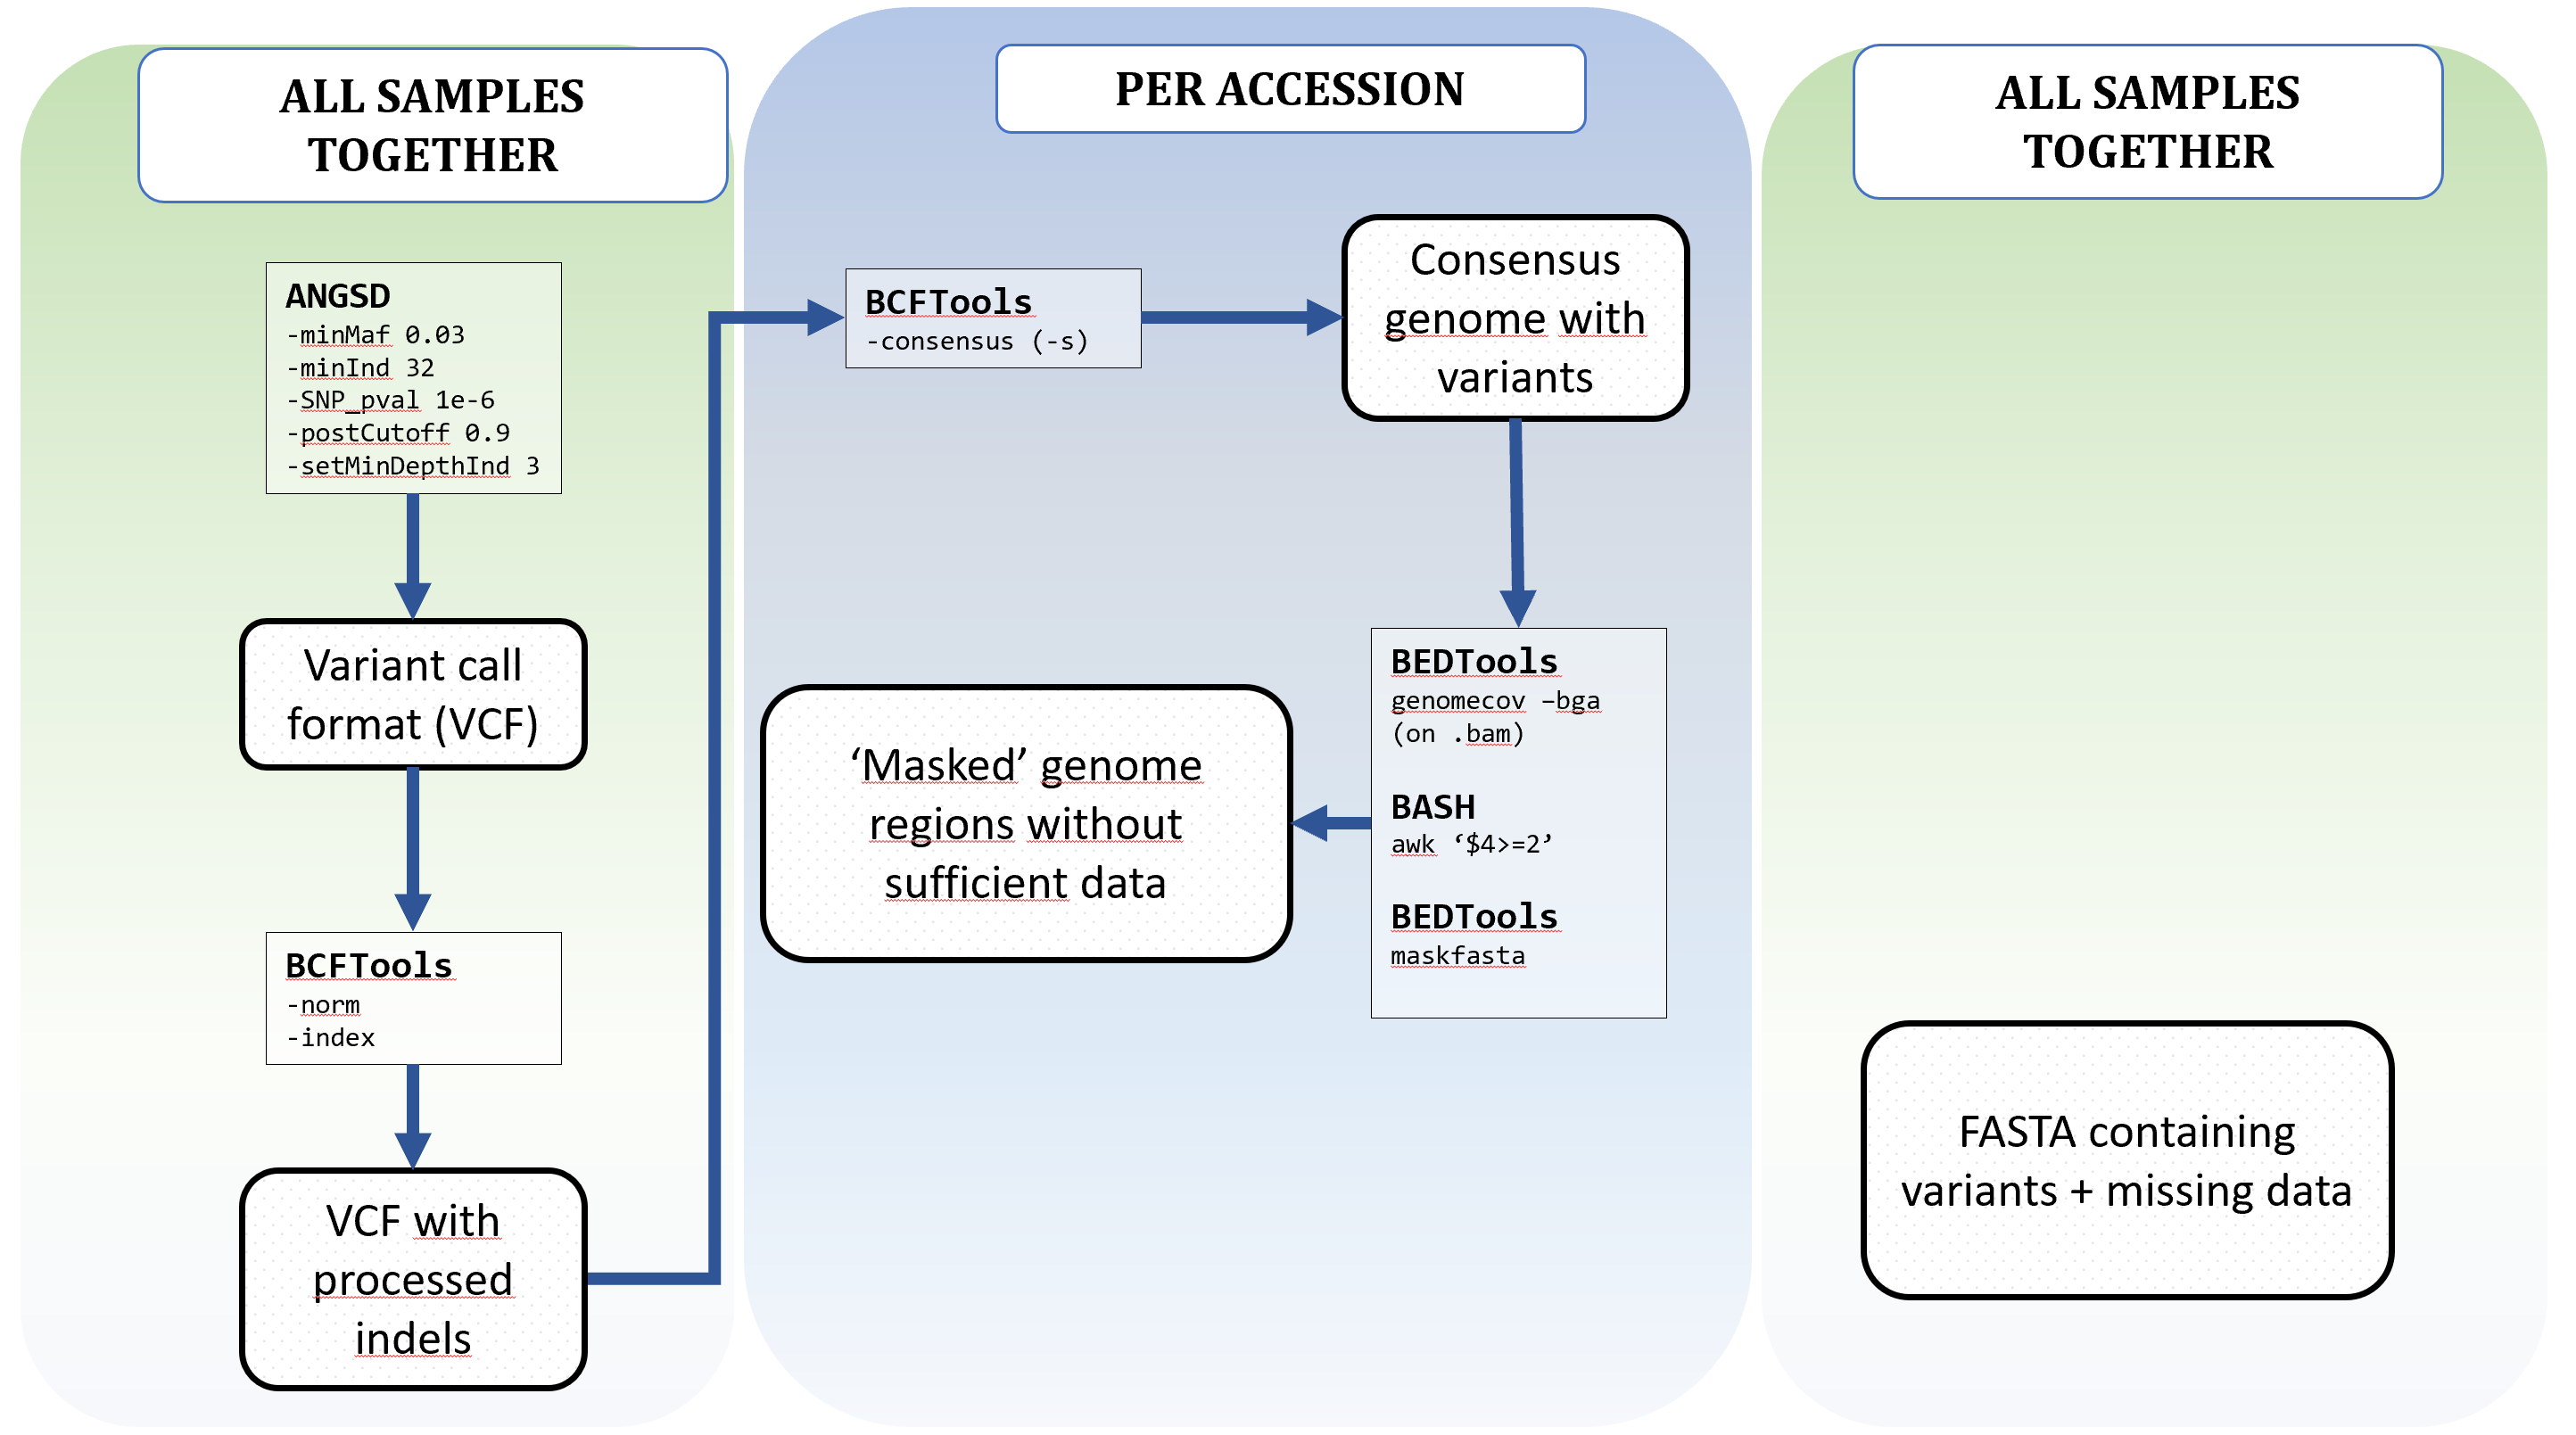
\includegraphics[height=6cm]{Images/alignment_workflow.PNG}
        \caption{Figure 1: A basic idea for a workflow to recover full genome ``alignments'' of all sequenced accessions using bam files. Note, this is not a traditional alignment in the sense that accession data was not pairwise-aligned; instead, the alignment of accessions stems from high-quality/stringency mapping to an identical reference sequence. \emph{This is still being refined.}}
\end{figure}

At the first hurdle, an issue was encountered. The bfctools ``consensus'' command requires that an indexed vcf/bcf file be used. Unfortunately, the output of ANGSD does not seem to directly meet these criteria. Indexing can simply be completed using the ``bgzip'' and ``tabix'' packages (see \url{https://www.biostars.org/p/367960/}) but these are not immediately available through the Nix repository. Instead, I will attempt to use an entirely bcftools-based approach suggested by user ``pd3'' at the following link: \url{https://github.com/samtools/bcftools/issues/668}. Essentially, this involved first converting the bcf file to a zipped vcf, and then indexing the zipped vcf file.

\begin{codewrap}
  > bcftools view /bettik/greenwom/WGS/Genotypes/coenonympha.bcf -Oz -o /bettik/greenwom/WGS/Genotypes/coenonympha.vcf.gz
  > bcftools index /bettik/greenwom/WGS/Genotypes/coenonympha.vcf.gz
\end{codewrap}

It may be important to consider also trimming the bam files to only have bases with read maps > 20 in terms of quality score before doing any of these consensus construction steps.

To see if the consensus contruction, variant insertion, and masking worked, I wrote a script (``6.3-GetGenomeAlignments'') to clip a stretch of bases off the first scaffold of each accession. This script will probably be a useful starting point for when I want to divide the genome up into windows for phylogenetic inference. The results of this clipping were visualized in SeaView version 5 \cite{galtier1996}. In general, the bam-centric sequence reconstruction process has produced long stretches of good-looking alignments. Of course, the ``cleaness'' of this alignment may be expected due to the consensus process used to generate full species sequences.

 Along a small sample of the genome (scaffold 1, position 2000000-2226000; 6001 bases), there are many examples of pristine low-diversity regions (e.g., Figure 2), as well as a few scattered islands housing interspecific diversity (e.g., Figure 3).  There are, also, a few areas with high levels of sequence drop-out (e.g., Figure 4); in the near future, it may be necessary to make use of trimAl \cite{capella2009} for defined pruning and reproducible of these gappy sections of species alignments.

 \begin{figure}[!h]
         \centering
         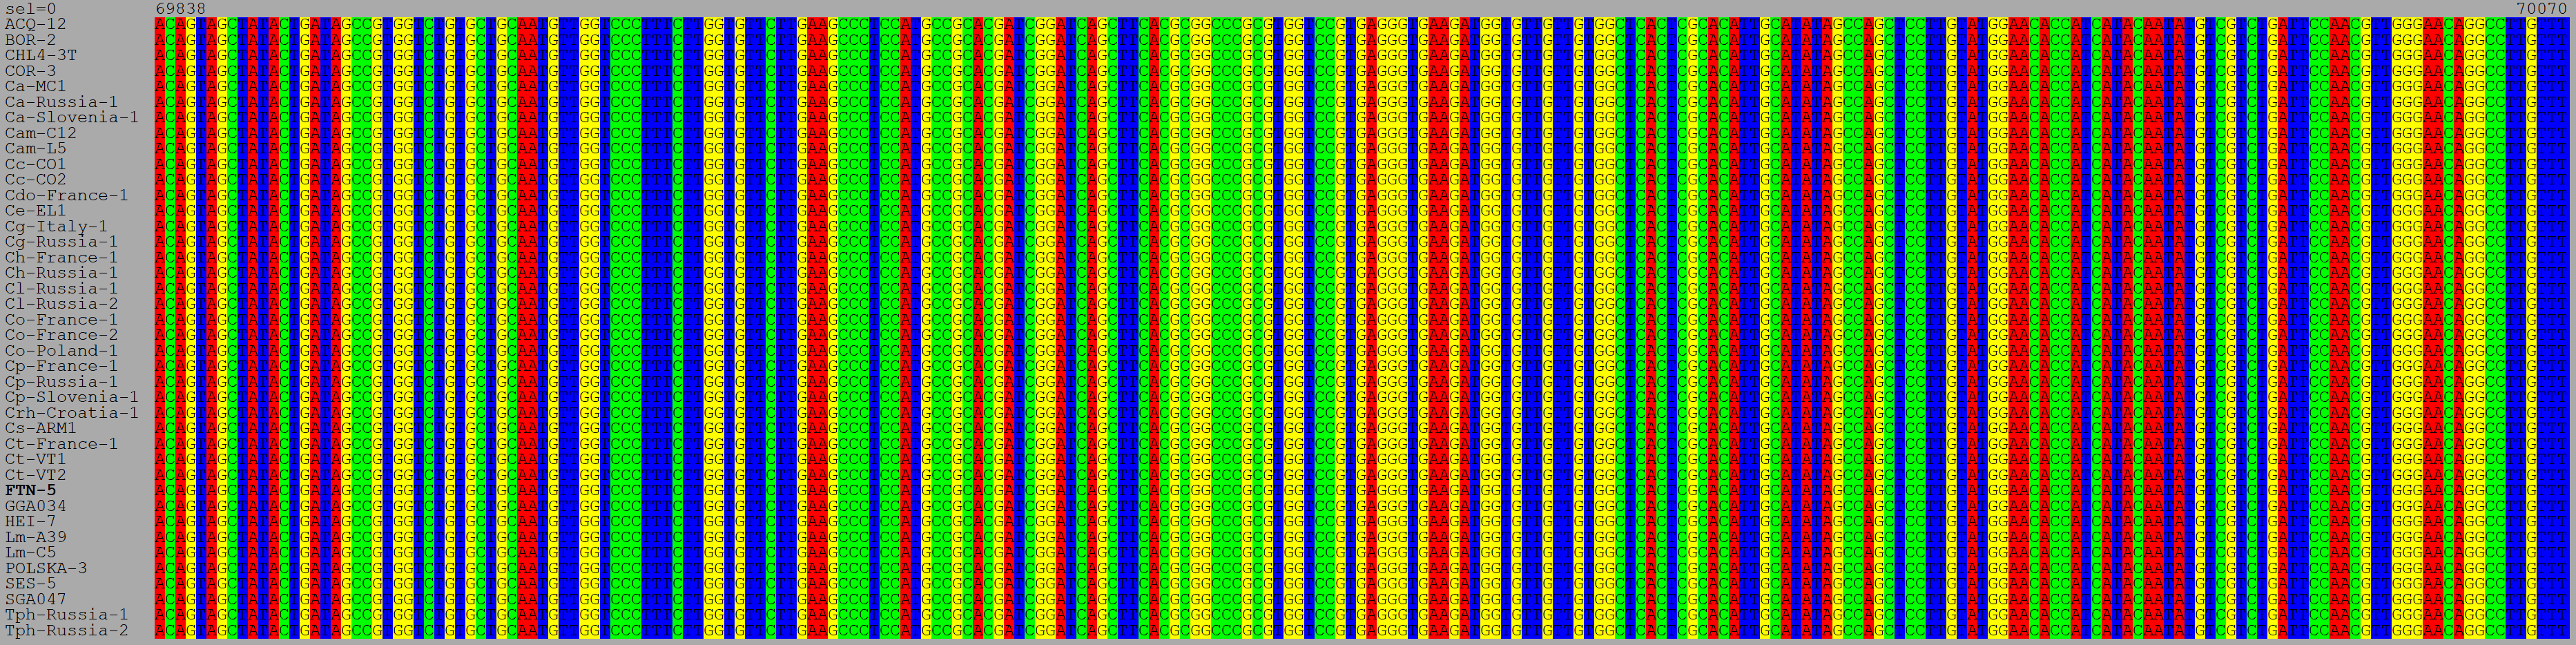
\includegraphics[height=4cm]{Images/SeaViewMSA_1.PNG}
         \caption{Figure 2: An example of low diversity genomic stretches which are common throught the multiple species alignment (MSA), at least for this considered genomic region.}
 \end{figure}

 \begin{figure}[!h]
         \centering
         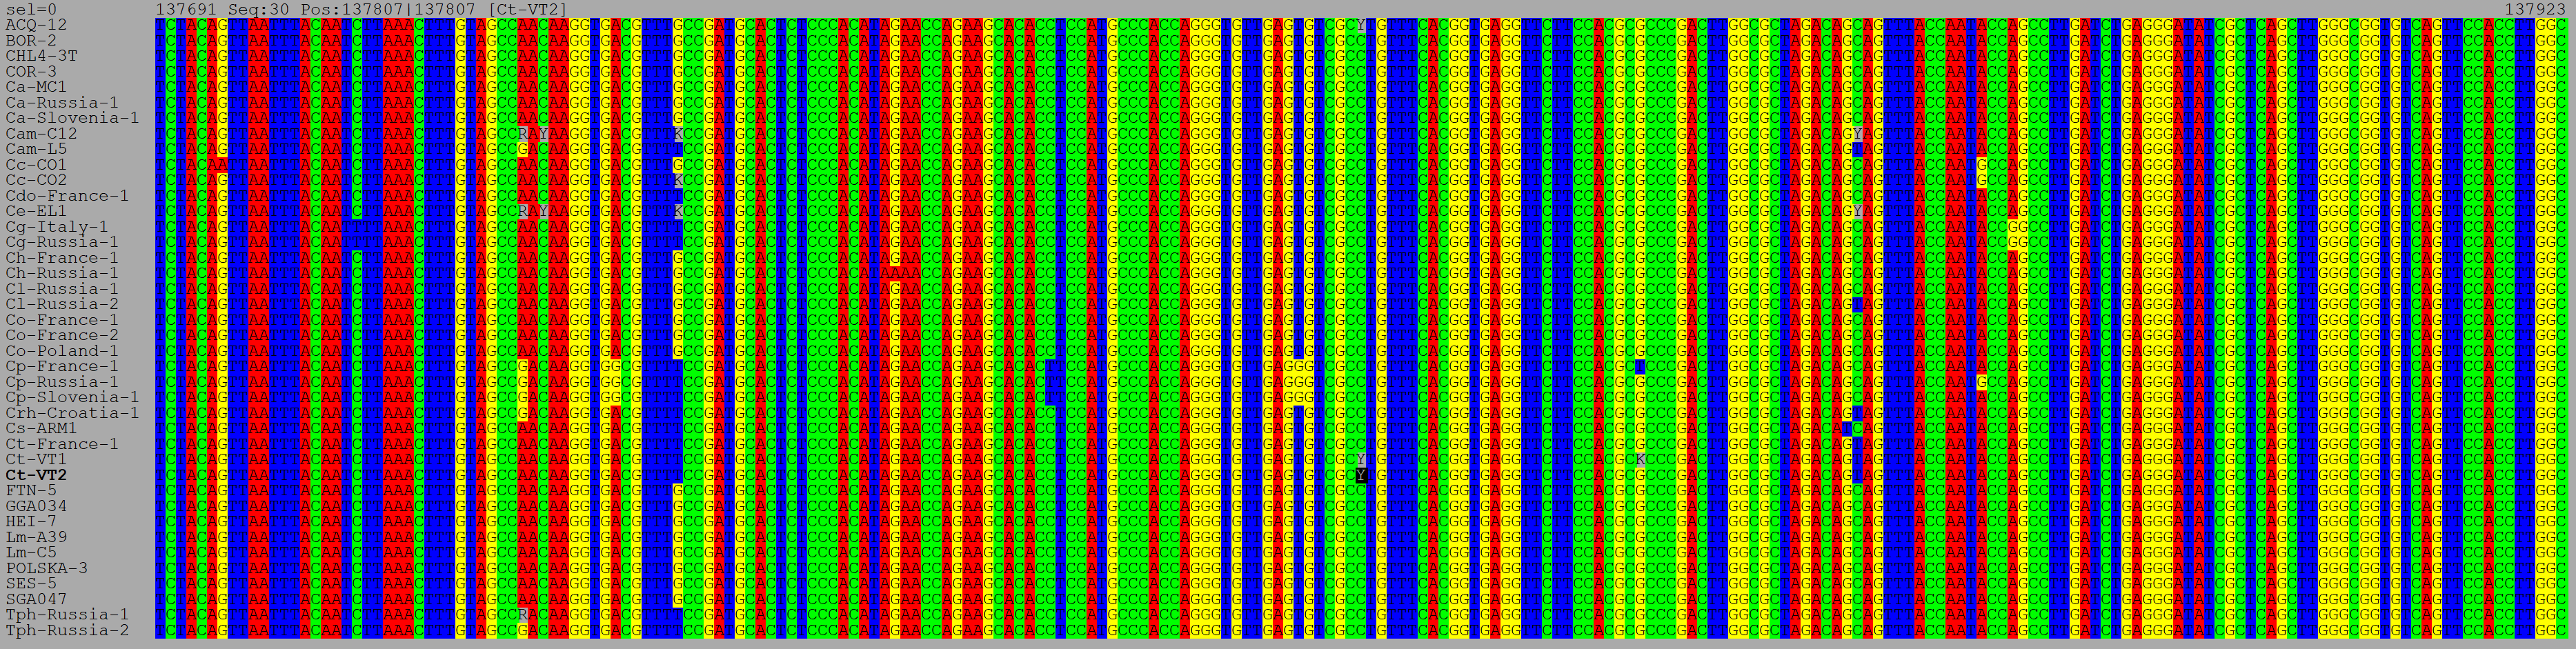
\includegraphics[height=4cm]{Images/SeaViewMSA_2.PNG}
         \caption{Figure 3: An example of sparse but high interspecific diversity genomic loci in the multiple species alignment (MSA), at least for this considered genomic region.}
 \end{figure}

 \begin{figure}[!h]
         \centering
         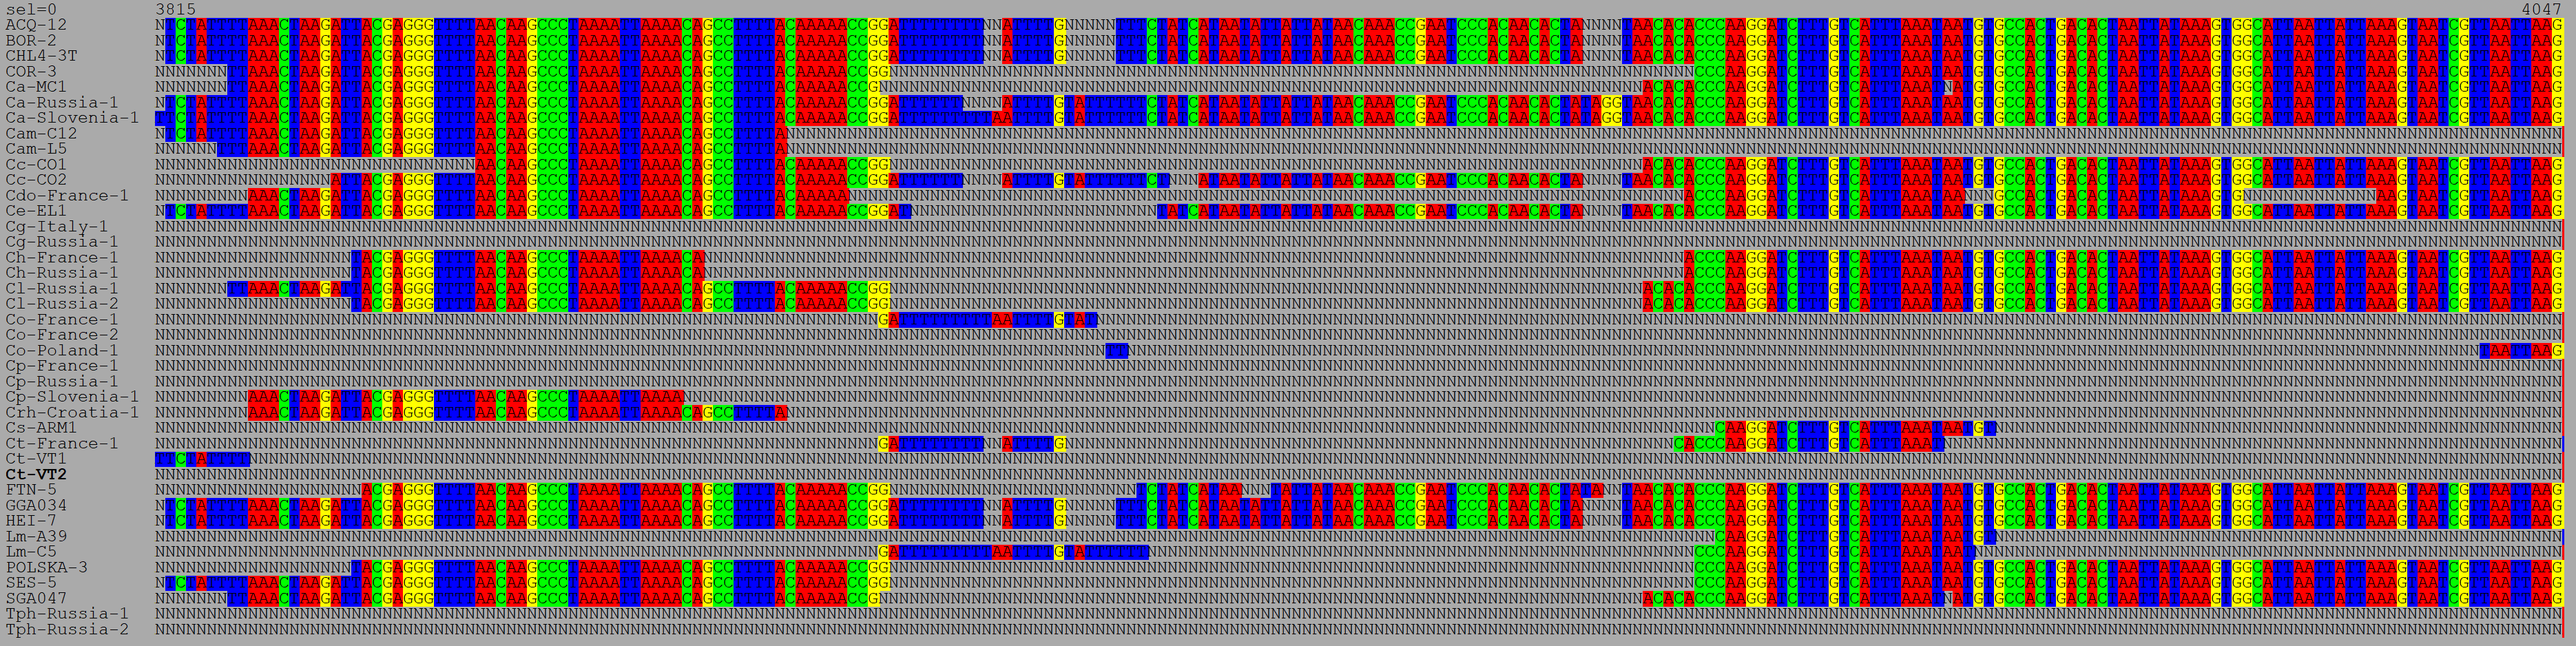
\includegraphics[height=4cm]{Images/SeaViewMSA_3.PNG}
         \caption{Figure 4: An example of reasonably common``gappy'' domains of the multiple species alignment (MSA), at least for this considered genomic region.}
 \end{figure}

I have split the scaffolds into abutting windows of 100000 bp (see scripts ``7.1-.sh'', ``7.2-.sh'', and ``7.3-SplitScaffoldsIntoAlignedWindows.sh'') that can be used to infer species topologies along scaffolds and assemble a consensus tree with ASTRAL III (ref). I plan to use trimAl to cut out gappy regions of these alignments. Then, I want to apply AMAS (ref) to determine the quality of trimmed alignments and to provide a metric for the filtering of useful alignments. In the process of reading up on AMAS, I've discovered it may be capable of splitting fastas into abutting windows, as is accomplished by my ``7.X'' series of scripts.  

Things still to do: filter by mapping quality before making consensus genomes; mask repeat regions. Also, it could be worthwhile to try less stringent ANGSD filtering; e.g., min allele frequency of \~0 and a lower minInd.

\bibliography{citations}



\end{document}
